\section{Профилирование ступени ТВД}
Исходными данными для данного этапа проектирования турбины являются результы расчета по средней линии тока.

Ступень была спрофилирована по закону $\alpha_1=const$.

Определим треугольники скоростей на произвольном радиусе лопатки.

\begin{enumerate}

	\item В этом случае значения абсолютной скорости на входе на рабочие лопатки на произвольном радиусе определялись по следующим формулам (в приведенных ниже формулах значения со штрихом относятся к среднему радиусу):
		$$
			c_{1u} = c_{1u}^\prime \left( \frac{r^\prime}{r} \right)^{cos^2\alpha}; \/\
			c_{1a} = c_{1a}^\prime \left( \frac{r^\prime}{r} \right)^{cos^2\alpha}; \/\
			c_1 = c_1^\prime \left( \frac{r^\prime}{r} \right)^{cos^2\alpha}
		$$

	\item Окружная скорость рабочей лопатки на произвольном радиусе была определена по закону вращения твердого тела:
		$$
			u = u^\prime \frac{r}{r^\prime}
		$$

	\item Относительная скорость на произвольном радиусе на входе в рабочие лопатки была определена по следующим формулам:
		$$
			w_{1u} = c_{1u} - u; \/\ 
			w_{1a} = c_{1a}; \/\ 
			w_1 = \sqrt{w_{1u}^2 + w_{1a}^2}
		$$

	\item Абсолютная скорость на выходе из рабочих лопаток была определена по условию постоянства работы, отводимой от газа на различных радиусах лопатки.

	По формуле Эйлера для правила отсчета углов, принятого в теории турбин удельная работа на окружности колеса $L_u$ определяется слеюущей формулой:
		$$
			L_u = c_{1u} + c_{2u}
		$$
	Таким образом, зная работу на окружности колеса на среднем радиусе лопатки $L_u^\prime$, мы можем определить значение окружной скорости на выходе из рабочих лопаток:
		$$
			c_{2u} = \frac{L_u^\prime}{u} - c_{1u} =
				\frac{L_u^\prime}{u^\prime} 
				\frac{r^\prime}{r} - 
				c_{1u}^\prime \left( 
					\frac{r^\prime}{r} 
				\right)^{cos^2\alpha_1} 
		$$

	\item Используя значения окружной и осевой скорости на среднем радиусе лопатки, определим значение осевой скорости на выходе из рабочих лопаток, проинтегрировав уравнение радиального равновесия:
		$$
			c_{2a}^2 = c_{2a}^{\prime 2} + c_{2u}^{\prime 2} - c_{2u}^{2} - 2 \int_{r^\prime}^r \frac{c_{2u}^2}{r} dr
		$$
%	Введем обозначения $a = \frac{L_u^\prime}{u}; \/\ b = c_{1u}^\prime$.
%
%	Тогда после интегрирования получим:
%		$$
%			c_{2a} = c_{2a}^{\prime 2} + c_{2u}^{\prime 2} - c_{2u}^{2} +
%			\left. \left[
%				- a^2 \left(
%					\frac{r^\prime}{r}
%				\right)^{2} +
%				\frac{4ab}{
%					1 + cos^2 \alpha_1
%				}\left(
%					\frac{r^\prime}{r}
%				\right)^{1 + \cos^2\alpha_1} -
%				\frac{b^2}{\cos^2 \alpha_1} \left(
%					\frac{r^\prime}{r}
%				\right)^{2cos^2 \alpha_1}
%			\right] \right|_{r^\prime}^r
%		$$

	\item Значения проекций относительной скорости на выходе из лопаток находим так же, как и значения на входе в рабочие лопатки.

%	Определим профили давления и реактивности на произвольном радиусе лопатки:
%	\begin{enumerate}
%		\item Запишем выражение для числа Маха на произвольном радиусе лопатки:
%		$$
%			M_{1, 2} = \frac{
%				c_{1,2}
%			}{
%				\sqrt{kR \left( T_{1, 2} + \frac{{c_{1,2}}^2 - {c_{1,2}^\prime}^2}{c_p} \right)}
%			}
%		$$
%		\item Запишем выражение для давления на произвольном радиусе лопатки, используя ГДФ давления:
%		$$
%			p_{1,2} = p_{1,2}^\prime \frac{
%				\pi(M_{1,2}^\prime), k
%			}{
%				\pi(M_{1,2}), k
%			}
%		$$
%		\item Запишем выражение для статической температура на произвольном радиусе лопатки, используя ГДФ давления:
%		$$
%			p_{1,2} = p_{1,2}^\prime \frac{
%				\pi(M_{1,2}^\prime), k
%			}{
%				\pi(M_{1,2}), k
%			}
%		$$
%	\end{enumerate}

\end{enumerate}

Распределение углов на входе в рабочие лопатки турбины и на выходе из них представлено на рис. 2 и 3, соответственно:
	\begin{figure}[H]
		\centering
		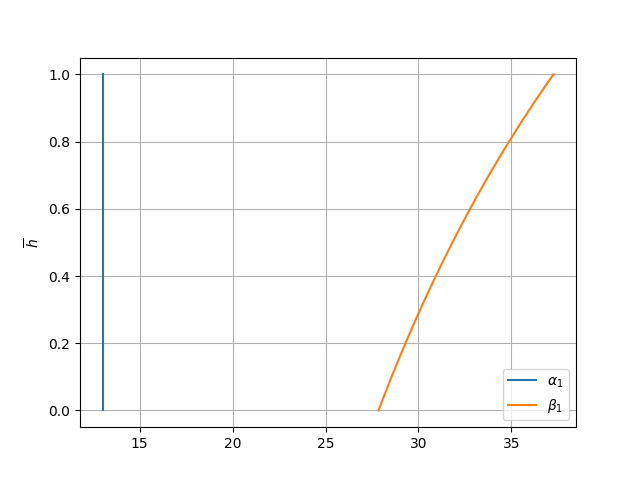
\includegraphics[scale=0.6]{inlet_angle}
		\caption{Углы на входе в лопатки турбины}
	\end{figure}

	\begin{figure}[H]
		\centering
		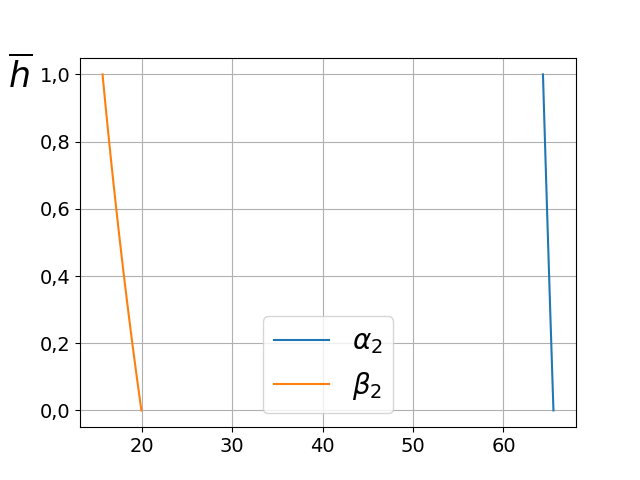
\includegraphics[scale=0.6]{outlet_angle}
		\caption{Углы на выходе из лопаток турбины}
	\end{figure}

%Ниже представлены профили лопаток статора и ротора на трех радиусах
%    \begin{figure}
%        \centering
%        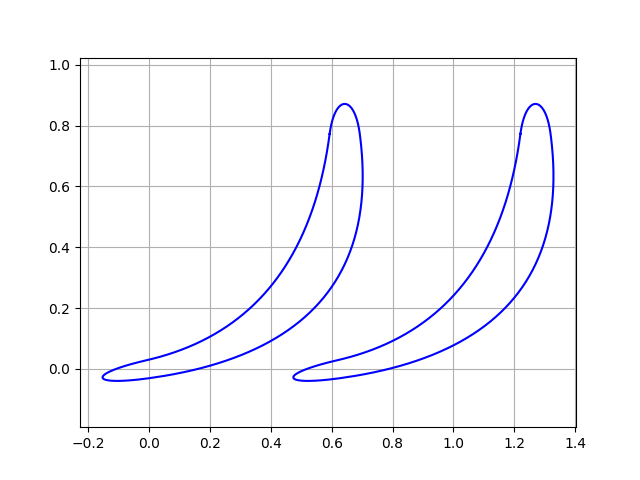
\includegraphics[scale=0.6]{stator_root}
%        \caption{Профиль статора на втулке}
%    \end{figure}
%
%    \begin{figure}
%        \centering
%        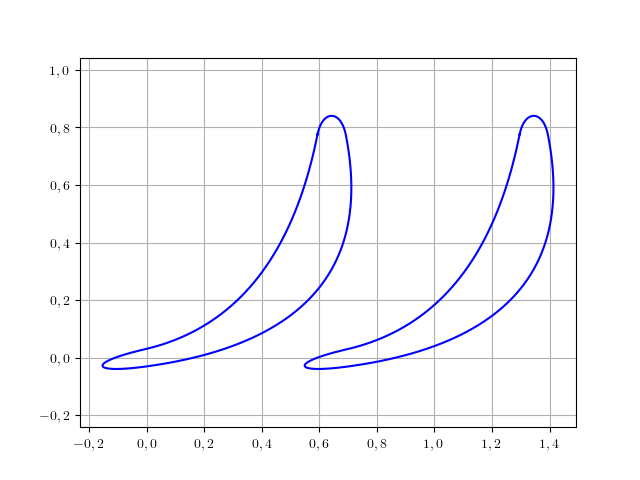
\includegraphics[scale=0.6]{stator_mid}
%        \caption{Профиль статора на среднем радиусе}
%    \end{figure}
%
%    \begin{figure}
%        \centering
%        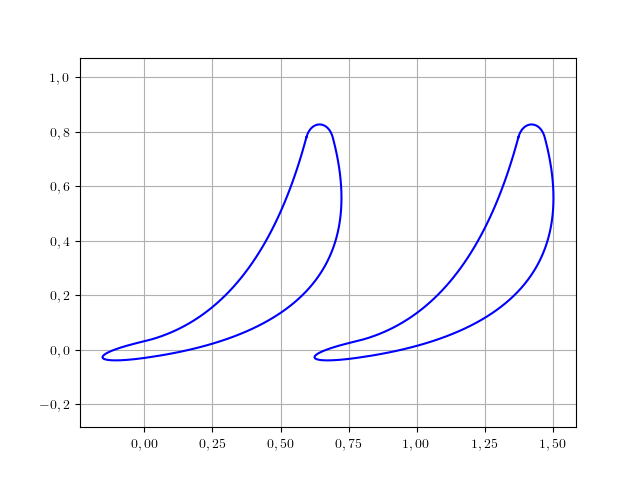
\includegraphics[scale=0.6]{stator_top}
%        \caption{Профиль статора на периферии}
%    \end{figure}
%
%    \begin{figure}
%        \centering
%        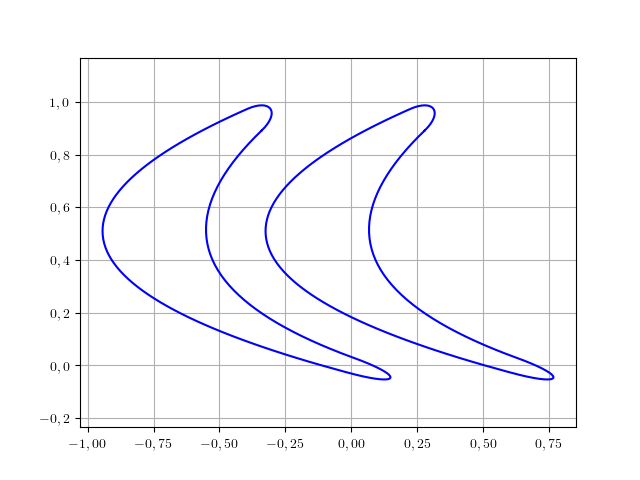
\includegraphics[scale=0.6]{rotor_root}
%        \caption{Профиль ротора на втулке}
%    \end{figure}
%
%    \begin{figure}
%        \centering
%        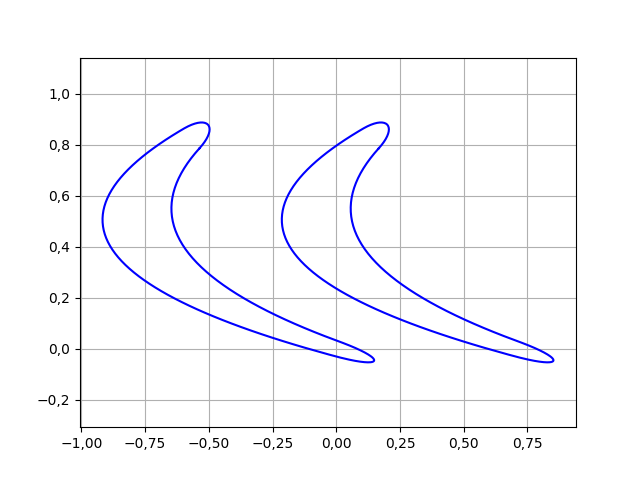
\includegraphics[scale=0.6]{rotor_mid}
%        \caption{Профиль ротора на среднем радиусе}
%    \end{figure}
%
%    \begin{figure}
%        \centering
%        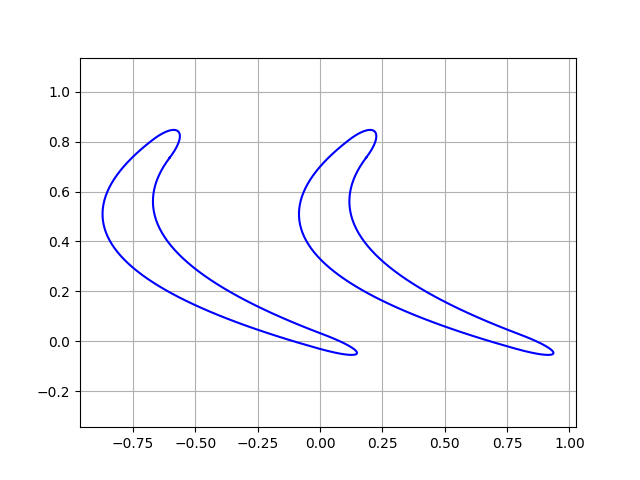
\includegraphics[scale=0.6]{rotor_top}
%        \caption{Профиль ротора на периферии}
%    \end{figure}
